% Created by tikzDevice version 0.12.3.2 on 2022-03-16 11:02:52
% !TEX encoding = UTF-8 Unicode
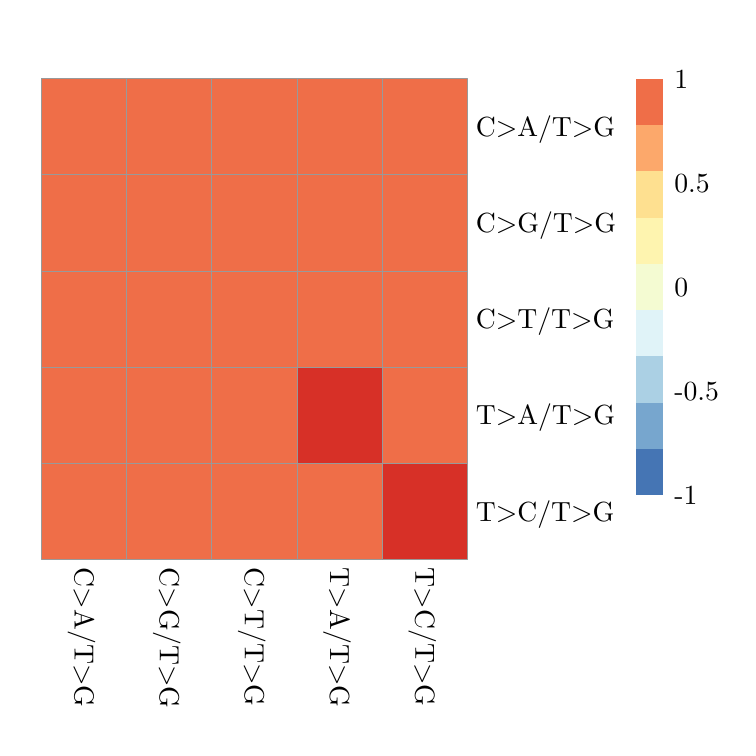
\begin{tikzpicture}[x=1pt,y=1pt]
\definecolor{fillColor}{RGB}{255,255,255}
\path[use as bounding box,fill=fillColor,fill opacity=0.00] (0,0) rectangle (252.94,252.94);
\begin{scope}
\path[clip] (  0.00,  0.00) rectangle (252.94,252.94);
\definecolor{drawColor}{gray}{0.60}
\definecolor{fillColor}{RGB}{239,110,72}

\path[draw=drawColor,line width= 0.4pt,line join=round,line cap=round,fill=fillColor] (  5.02,199.74) rectangle ( 35.80,234.50);

\path[draw=drawColor,line width= 0.4pt,line join=round,line cap=round,fill=fillColor] (  5.02,164.99) rectangle ( 35.80,199.74);

\path[draw=drawColor,line width= 0.4pt,line join=round,line cap=round,fill=fillColor] (  5.02,130.23) rectangle ( 35.80,164.99);

\path[draw=drawColor,line width= 0.4pt,line join=round,line cap=round,fill=fillColor] (  5.02, 95.48) rectangle ( 35.80,130.23);

\path[draw=drawColor,line width= 0.4pt,line join=round,line cap=round,fill=fillColor] (  5.02, 60.72) rectangle ( 35.80, 95.48);

\path[draw=drawColor,line width= 0.4pt,line join=round,line cap=round,fill=fillColor] ( 35.80,199.74) rectangle ( 66.58,234.50);

\path[draw=drawColor,line width= 0.4pt,line join=round,line cap=round,fill=fillColor] ( 35.80,164.99) rectangle ( 66.58,199.74);

\path[draw=drawColor,line width= 0.4pt,line join=round,line cap=round,fill=fillColor] ( 35.80,130.23) rectangle ( 66.58,164.99);

\path[draw=drawColor,line width= 0.4pt,line join=round,line cap=round,fill=fillColor] ( 35.80, 95.48) rectangle ( 66.58,130.23);

\path[draw=drawColor,line width= 0.4pt,line join=round,line cap=round,fill=fillColor] ( 35.80, 60.72) rectangle ( 66.58, 95.48);

\path[draw=drawColor,line width= 0.4pt,line join=round,line cap=round,fill=fillColor] ( 66.58,199.74) rectangle ( 97.36,234.50);

\path[draw=drawColor,line width= 0.4pt,line join=round,line cap=round,fill=fillColor] ( 66.58,164.99) rectangle ( 97.36,199.74);

\path[draw=drawColor,line width= 0.4pt,line join=round,line cap=round,fill=fillColor] ( 66.58,130.23) rectangle ( 97.36,164.99);

\path[draw=drawColor,line width= 0.4pt,line join=round,line cap=round,fill=fillColor] ( 66.58, 95.48) rectangle ( 97.36,130.23);

\path[draw=drawColor,line width= 0.4pt,line join=round,line cap=round,fill=fillColor] ( 66.58, 60.72) rectangle ( 97.36, 95.48);

\path[draw=drawColor,line width= 0.4pt,line join=round,line cap=round,fill=fillColor] ( 97.36,199.74) rectangle (128.14,234.50);

\path[draw=drawColor,line width= 0.4pt,line join=round,line cap=round,fill=fillColor] ( 97.36,164.99) rectangle (128.14,199.74);

\path[draw=drawColor,line width= 0.4pt,line join=round,line cap=round,fill=fillColor] ( 97.36,130.23) rectangle (128.14,164.99);
\definecolor{fillColor}{RGB}{215,48,39}

\path[draw=drawColor,line width= 0.4pt,line join=round,line cap=round,fill=fillColor] ( 97.36, 95.48) rectangle (128.14,130.23);
\definecolor{fillColor}{RGB}{239,110,72}

\path[draw=drawColor,line width= 0.4pt,line join=round,line cap=round,fill=fillColor] ( 97.36, 60.72) rectangle (128.14, 95.48);

\path[draw=drawColor,line width= 0.4pt,line join=round,line cap=round,fill=fillColor] (128.14,199.74) rectangle (158.92,234.50);

\path[draw=drawColor,line width= 0.4pt,line join=round,line cap=round,fill=fillColor] (128.14,164.99) rectangle (158.92,199.74);

\path[draw=drawColor,line width= 0.4pt,line join=round,line cap=round,fill=fillColor] (128.14,130.23) rectangle (158.92,164.99);

\path[draw=drawColor,line width= 0.4pt,line join=round,line cap=round,fill=fillColor] (128.14, 95.48) rectangle (158.92,130.23);
\definecolor{fillColor}{RGB}{215,48,39}

\path[draw=drawColor,line width= 0.4pt,line join=round,line cap=round,fill=fillColor] (128.14, 60.72) rectangle (158.92, 95.48);
\end{scope}
\begin{scope}
\path[clip] (  0.00,  0.00) rectangle (252.94,252.94);
\definecolor{drawColor}{RGB}{0,0,0}

\node[text=drawColor,rotate=270.00,anchor=base west,inner sep=0pt, outer sep=0pt, scale=  1.00] at ( 16.96, 57.71) {C$>$A/T$>$G};

\node[text=drawColor,rotate=270.00,anchor=base west,inner sep=0pt, outer sep=0pt, scale=  1.00] at ( 47.74, 57.71) {C$>$G/T$>$G};

\node[text=drawColor,rotate=270.00,anchor=base west,inner sep=0pt, outer sep=0pt, scale=  1.00] at ( 78.52, 57.71) {C$>$T/T$>$G};

\node[text=drawColor,rotate=270.00,anchor=base west,inner sep=0pt, outer sep=0pt, scale=  1.00] at (109.30, 57.71) {T$>$A/T$>$G};

\node[text=drawColor,rotate=270.00,anchor=base west,inner sep=0pt, outer sep=0pt, scale=  1.00] at (140.08, 57.71) {T$>$C/T$>$G};
\end{scope}
\begin{scope}
\path[clip] (  0.00,  0.00) rectangle (252.94,252.94);
\definecolor{drawColor}{RGB}{0,0,0}

\node[text=drawColor,anchor=base west,inner sep=0pt, outer sep=0pt, scale=  1.00] at (161.93,213.68) {C$>$A/T$>$G};

\node[text=drawColor,anchor=base west,inner sep=0pt, outer sep=0pt, scale=  1.00] at (161.93,178.92) {C$>$G/T$>$G};

\node[text=drawColor,anchor=base west,inner sep=0pt, outer sep=0pt, scale=  1.00] at (161.93,144.17) {C$>$T/T$>$G};

\node[text=drawColor,anchor=base west,inner sep=0pt, outer sep=0pt, scale=  1.00] at (161.93,109.41) {T$>$A/T$>$G};

\node[text=drawColor,anchor=base west,inner sep=0pt, outer sep=0pt, scale=  1.00] at (161.93, 74.66) {T$>$C/T$>$G};
\end{scope}
\begin{scope}
\path[clip] (  0.00,  0.00) rectangle (252.94,252.94);
\definecolor{fillColor}{RGB}{69,117,180}

\path[fill=fillColor] (219.64, 83.93) rectangle (229.68,100.66);
\definecolor{fillColor}{RGB}{119,166,206}

\path[fill=fillColor] (219.64,100.66) rectangle (229.68,117.39);
\definecolor{fillColor}{RGB}{171,208,228}

\path[fill=fillColor] (219.64,117.39) rectangle (229.68,134.12);
\definecolor{fillColor}{RGB}{224,243,248}

\path[fill=fillColor] (219.64,134.12) rectangle (229.68,150.85);
\definecolor{fillColor}{RGB}{244,251,210}

\path[fill=fillColor] (219.64,150.85) rectangle (229.68,167.58);
\definecolor{fillColor}{RGB}{254,244,175}

\path[fill=fillColor] (219.64,167.58) rectangle (229.68,184.31);
\definecolor{fillColor}{RGB}{254,224,144}

\path[fill=fillColor] (219.64,184.31) rectangle (229.68,201.04);
\definecolor{fillColor}{RGB}{252,168,107}

\path[fill=fillColor] (219.64,201.04) rectangle (229.68,217.77);
\definecolor{fillColor}{RGB}{239,110,72}

\path[fill=fillColor] (219.64,217.77) rectangle (229.68,234.50);
\definecolor{drawColor}{RGB}{0,0,0}

\node[text=drawColor,anchor=base west,inner sep=0pt, outer sep=0pt, scale=  1.00] at (233.69, 80.49) {-1};

\node[text=drawColor,anchor=base west,inner sep=0pt, outer sep=0pt, scale=  1.00] at (233.69,118.13) {-0.5};

\node[text=drawColor,anchor=base west,inner sep=0pt, outer sep=0pt, scale=  1.00] at (233.69,155.77) {0};

\node[text=drawColor,anchor=base west,inner sep=0pt, outer sep=0pt, scale=  1.00] at (233.69,193.41) {0.5};

\node[text=drawColor,anchor=base west,inner sep=0pt, outer sep=0pt, scale=  1.00] at (233.69,231.05) {1};
\end{scope}
\end{tikzpicture}
